\section{Particle-mesh method}
The particle-mesh method can be described as the following sequence of four steps:
\begin{enumerate}
    \item Assign masses to mesh points,
    \item Solve the field equation (\autoref{eq:poisson}) on the mesh,
    \item Calculate the field strength at mesh-points,
    \item Find forces applied to individual particles by interpolation.
\end{enumerate}
In this section, each of these steps will be described in more detail.

\subsection{Mass assignment}\label{subsec:mass-assignment}
The specifics of assigning mass from particles to mesh points depend on the density profile (or \textit{shape}) associated with the particles.
In general, the particles need not be represented as idealized dimensionless points;
indeed, it is possible to construct a hierarchy of shapes, where each successive member covers a larger number of mesh points and whose application leads to smaller numerical errors.

An infinite hierarchy of shapes with this property, as described by Hockney and Eastwood in \cite{Hockney1988}, can be generated by successive convolutions with the ``top-hat'' function $\Pi$, defined as
\begin{equation*}
    \Pi(x) = \begin{cases}
        1,           & |x| < \frac{1}{2} \\
        \frac{1}{2}, & |x| = 1           \\
        0,           & \text{otherwise}.
    \end{cases}
\end{equation*}
The three most popular assignment schemes that hail from this family (and the ones implemented in our program) are the \textit{nearest grid point} (NGP), \textit{cloud in cell} (CIC), and \textit{triangular shaped cloud} (TSC) schemes, with shapes $S$ given by
\begin{align*}
    S_\text{NGP} & = \delta(x), & S_\text{CIC} & = \delta(x) * \frac{1}{H} \Pi\left(\frac{x}{H}\right) = \frac{1}{H}\Pi\left(\frac{x}{H}\right), & S_\text{TSC} & = \frac{1}{H}\Pi\left(\frac{x}{H}\right) * \frac{1}{H}\Pi\left(\frac{x}{H}\right) = \frac{1}{H}\Lambda \left(\frac{x}{H}\right),
\end{align*}
where $\Lambda$ is the triangle function
\begin{equation*}
    \Lambda(x) = \begin{cases}
        1 - |x|, & |x| < 1           \\
        0,       & \text{otherwise}.
    \end{cases}
\end{equation*}
For illustrative purposes, the shape $S_\text{CIC}$ is depicted in \autoref{fig:cic-shape}.
\begin{figure}[htp]
    \centering
    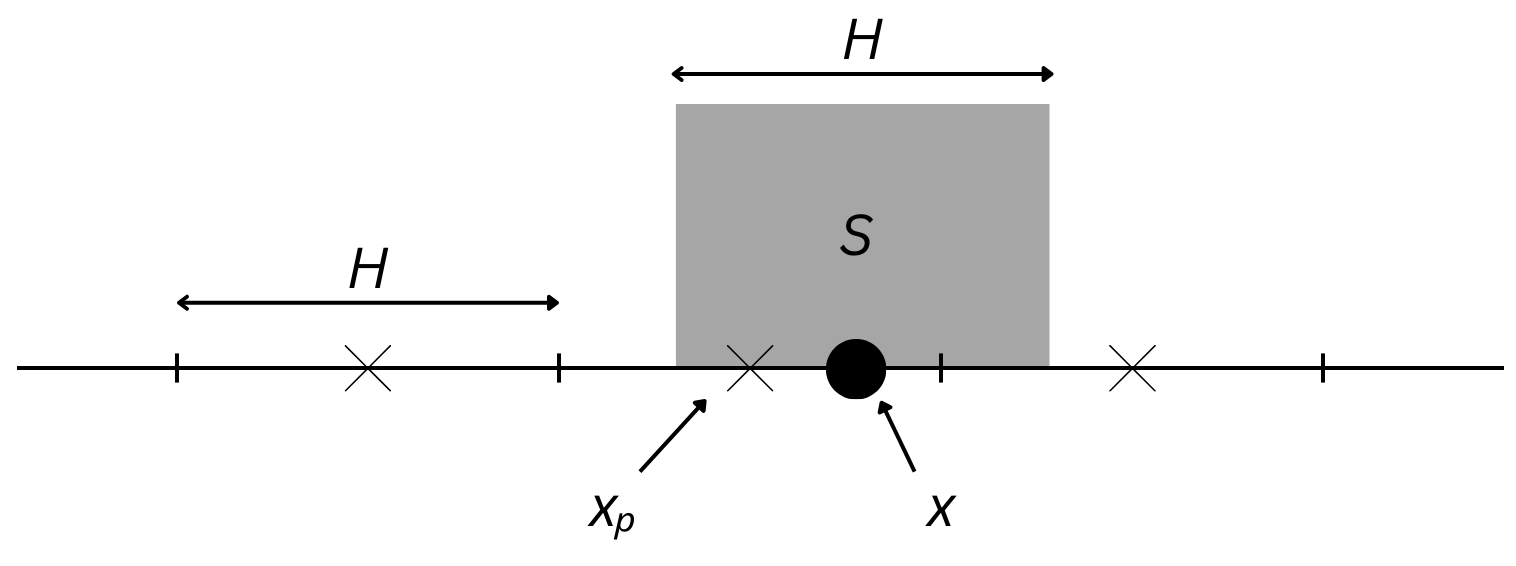
\includegraphics[scale=0.2]{img/CIC.png}
    \caption{The CIC shape centered at $x$ (particle position).
        The particle is within cell $x_p$, however, the cell $x_{p+1}$ gets non-zero density contribution from the particle.}
    \label{fig:cic-shape}
\end{figure}

In the one-dimensional case, the fraction of mass $W_p$ assigned to mesh-point $p$ from particle at position $x$ is given by
\begin{equation*}
    W(x-x_p) = W_p(x) = \int_{x_p-H/2}^{x_p+H/2} S(x'-x)dx'.
\end{equation*}
A simple rule for relating the assignment function $W$ defined above with shape $S$ can be found by noticing that
\begin{equation*}
    W(x) = \int_{-H/2}^{H/2}S(x'-x)dx' = \int_{-\infty}^\infty \Pi\left(\frac{x'}{H}\right)S(x'-x)dx' = \Pi\left(\frac{x}{H}\right) * S(x).
\end{equation*}
This implies that
\begin{align}\label{eq:assignment-functions}
    W_\text{NGP}(x) & = \Pi\left(\frac{x}{H}\right), & W_\text{CIC}(x) & = \Lambda\left(\frac{x}{H}\right), & W_\text{TSC}(x) & = \Pi\left(\frac{x}{H}\right) * \frac{1}{H} \Lambda\left(\frac{x}{H}\right) = (\Pi * \Lambda)\left(\frac{x}{H}\right).
\end{align}
Splitting the domain of integration in the expression for $W_\text{TSC}$ into five disjoint intervals shows that
\begin{equation*}
    (\Pi * \Lambda)(x) = \begin{cases}
        \frac{1}{8}(3-2|x|)^2, & \frac{1}{2} \leq |x| < \frac{3}{2} \\
        \frac{3}{4}-x^2,       & |x| < \frac{1}{2}                  \\
        0,                     & \text{otherwise}.
    \end{cases}
\end{equation*}

Two- and three-dimensional versions of the assignment functions in \autoref{eq:assignment-functions} are products of the assignment functions in each dimension.
For example, the three-dimensional assignment function $W$ is
\begin{equation*}
    W(\mathbf{x}) = W(x)W(y)W(z).
\end{equation*}
Hence, the mass assigned at mesh-point at $\mathbf{x}_\mathbf{p}$ is
\begin{equation*}
    m(\mathbf{x}_\mathbf{p}) = \sum_i m_i W_\mathbf{p}(\mathbf{x}_i),
\end{equation*}
or, in terms of density $\rho$,
\begin{equation}\label{eq:density-assignment}
    \rho(\mathbf{x}_\mathbf{p}) = \frac{1}{V} \sum_i m_i W_\mathbf{p}(\mathbf{x}_i),
\end{equation}
where $V = H^3$ is the volume of a cell and $i$ indexes the particles.

Obviously, \autoref{eq:density-assignment} is not suitable for direct application in the actual algorithm.
Instead, we iterate over all particles, identify the parent cell $\mathbf{p}$ of each particle (and its neighborhood) and update $\rho$.
This process is illustrated in \autoref{alg:density-assignment}.
\begin{algorithm}
    \caption{Density assignment algorithm}\label{alg:density-assignment}
    \begin{algorithmic}[1]
        \ForAll {particle $i$}
        \ForAll {cell $\mathbf{q}$ in $\mathcal{C}_S(\mathbf{x}_i)$}
        \State $\rho(\mathbf{x}_\mathbf{q}) \gets \rho(\mathbf{x}_\mathbf{q}) + m_i W(\mathbf{x}_i - \mathbf{x}_\mathbf{q}) / V$
        \EndFor
        \EndFor
    \end{algorithmic}
\end{algorithm}
The set $\mathcal{C}_S(\mathbf{x}_i)$ of cells that have to be considered while assigning density from the $i$-th particle, depends on the shape $S$ of the particle.
Specifically, we have $\mathcal{C}_\mathrm{NGP}(\mathbf{x}) = \{[\mathbf{x} / H]\}$, $\mathcal{C}_\mathrm{CIC}(\mathbf{x}) = \{\lfloor \mathbf{x}/H \rfloor + \mathbf{t} \;|\; t_i =0,1\}$, and $\mathcal{C}_\mathrm{TSC}(\mathbf{x}) = \{[\mathbf{x} / H] + \mathbf{t} \;|\; t_i = -1, 0, 1\}$.
It follows that $|\mathcal{C}_\mathrm{NGP}(\mathbf{x})| = 1$, $|\mathcal{C}_\mathrm{CIC}(\mathbf{x})| = 8$, and $|\mathcal{C}_\mathrm{TSC}(\mathbf{x})| = 27$ which illustrates the increasing computational cost resulting from using higher-order assignment schemes.
We note that \autoref{alg:density-assignment} can be parallelized if atomic increments are used in line 3.

\subsection{Solving the field equation}\label{subsec:solving-the-field-equation}
The Poisson equation (\autoref{eq:poisson}) can be restated in integral form
\begin{equation*}
    \phi(\mathbf{x}) = \int \mathcal{G}(\mathbf{x}-\mathbf{x}')\rho(\mathbf{x}') dV',
\end{equation*}
which has the following discrete analogue
\begin{equation}\label{eq:poisson-discrete}
    \phi(\mathbf{x}_\mathbf{p}) = V \sum_{\mathbf{p}'} \mathcal{G}(\mathbf{x}_\mathbf{p} - \mathbf{x}_{\mathbf{p}'}) \rho(\mathbf{x}_{\mathbf{p}'}),
\end{equation}
where $\mathcal{G}$ is the Green's function (potential due to unit mass).
The right-hand side of \autoref{eq:poisson-discrete} is a convolution sum that runs over a finite set of mesh points.
If we assume periodic boundary conditions, we can apply the discrete Fourier transform to both sides and use the convolution theorem to conclude that\footnote{
    In this work, the Hockney \& Eastwood definition of DFT is used, i.e.
    \begin{equation*}
        D(x_p) = \frac{1}{L}\sum_{l=0}^{N-1}\hat{D}(k)e^{ikx_p}, \quad \hat{D}(k) = H\sum_{p=0}^{N-1}D(x_p)e^{-ikx_p},
    \end{equation*}
    where $x_p = pH$.
    The conversion between this form and another popular definition,
    \begin{equation}\label{eq:standard-dft}
        \widetilde{D_H}(k) = \sum_{p=0}^{N-1}D_H(p)e^{-i2\pi kp / N},
    \end{equation}
    is given by
    \begin{equation*}
        \widetilde{D_H}(k) = \frac{1}{H}\hat{D}\left(\frac{2\pi}{NH}k\right),
    \end{equation*}
    where $D_H(p) = D(pH)$.
}
\begin{equation}\label{eq:poisson-fourier-product}
    \hat{\phi}(\mathbf{k}) = \hat{\mathcal{G}}(\mathbf{k}) \hat{\rho}(\mathbf{k}).
\end{equation}

An approximation to $\hat{\mathcal{G}}$ can be found using a discretized version of the Laplacian in \autoref{eq:poisson-discrete}.
Specifically, for a 7-point stencil,
\begin{equation*}
    \begin{split}
        4\pi G\rho(\mathbf{x}_{ijk})
         & =\frac{\phi(\mathbf{x}_{i-1,j,k}) - 2\phi(\mathbf{x}_{ijk})+\phi(\mathbf{x}_{i+1,j,k})}{H^2}   \\
         & + \frac{\phi(\mathbf{x}_{i,j-1,k}) - 2\phi(\mathbf{x}_{ijk})+\phi(\mathbf{x}_{i,j+1,k})}{H^2}  \\
         & + \frac{\phi(\mathbf{x}_{i,j,k-1}) - 2\phi(\mathbf{x}_{ijk})+\phi(\mathbf{x}_{i,j,k+1})}{H^2}.
    \end{split}.
\end{equation*}
Applying the discrete Fourier transform to both sides and using the shift theorem we get
\begin{align*}
    4\pi G \hat{\rho}(\mathbf{k})
     & = \frac{1}{H^2}\sum_{i=1}^{3}\left( e^{-iHk_i} + e^{iHk_i}-2 \right)\hat{\phi}(\mathbf{k})       \\
     & = \frac{1}{H^2} \sum_{i=1}^{3}\left( e^{iHk_i/2} - e^{-iHk_i/2} \right)^2 \hat{\phi}(\mathbf{k}) \\
     & = -\frac{4}{H^2}\sum_{i=1}^{3}\sin^2\left(\frac{Hk_i}{2}\right)\hat{\phi}(\mathbf{k}).
\end{align*}
and hence
\begin{equation}\label{eq:dft-transformed-phi}
    \hat{\phi}(\mathbf{k}) = -4\pi G\underbrace{\frac{(H/2)^2}{\sin^2(Hk_1/2) + \sin^2(Hk_2/2) + \sin^2 (Hk_3/2)}}_{\hat{\mathcal{G}}(\mathbf{k})} \hat{\rho}(\mathbf{k}),
\end{equation}
where $\hat{\mathcal{G}}$ can be identified by comparison with \autoref{eq:poisson-fourier-product}.
It is worth noting that the constant multiplier $(-4\pi G)$ is often left out of $\hat{\mathcal{G}}$ (this is the convention used in \cite{Hockney1988}).
In the implementation, values of $\hat{\mathcal{G}}$ are computed only once and saved for future look-up.

In the one-dimensional case, the above discussion can be easily rephrased in terms of a diagonalization problem \cite{demanet2013fourier}.
In one dimension, the Poisson equation is
\begin{equation}\label{eq:poisson-1d}
    \frac{d^2 \phi}{dx^2} = \rho.
\end{equation}
The interval $[a, b]$ on which we wish to find $\phi$ is assumed to be discretized into $N$ points $x_j = a + jH$, where $H = (b - a) / (N - 1)$ and $j=0,\dots, N-1$.
Furthermore, we assume periodic boundary conditions so that $\phi(x_{-1}) = \phi(x_{N-1})$ and $\phi(x_{N}) = \phi(x_0)$.
The approximation of $\Delta$ at $x_j$ is
\begin{equation*}
    (\Delta_H \phi)_j \equiv \frac{\phi_{j-1} - 2\phi_j + \phi_{j+1}}{H^2}.
\end{equation*}
Thus, the discrete version of \autoref{eq:poisson-1d} reads $(\Delta_H \phi)_j = \rho_j$ or
\begin{equation*}
    \frac{\phi_{j-1}-2\phi_j + \phi_{j+1}}{H^2} = \rho_j,
\end{equation*}
where $\rho_j = \rho(x_j)$.
This gives a system of $N$ equations (one per each sampled value of $\rho$) with $N$ unknowns (values of $\phi$) of the following form
\begin{equation}\label{eq:poisson-1d-matrix}
    \underbrace{\frac{1}{H^2}
        \begin{bmatrix}
            2  & -1     &        &        & -1 \\
            -1 & 2      & \ddots &        &    \\
               & \ddots & \ddots & \ddots &    \\
               &        & \ddots & 2      & -1 \\
            -1 &        &        & -1     & 2
        \end{bmatrix}}_{\Delta_H}
    \underbrace{\begin{bmatrix}
            \phi_0     \\
            \phi_1     \\
            \vdots     \\
            \phi_{N-2} \\
            \phi_{N-1}
        \end{bmatrix}}_{\bar{\phi}}
    = -\underbrace{\begin{bmatrix}
            \rho_0     \\
            \rho_1     \\
            \vdots     \\
            \rho_{N-2} \\
            \rho_{N-1}
        \end{bmatrix}}_{\bar{\rho}}.
\end{equation}
Next we define $\bar{\psi}(k) \in \mathbb{C}^N$ by $\psi_j(k) \equiv e^{i2\pi jk/N} = \omega^{jk}$ for $j=0,\dots,N-1$.
The $j$-th row of $H^2\Delta_H \bar{\psi}$ equals
\begin{align*}
    (H^2\Delta_H \bar{\psi})_j
     & = -\psi_{j-1} + 2\psi_j - \psi_{j+1}
    = -\omega^{(j-1)k} + 2\omega^{jk} - \omega^{(j+1)k}     \\
     & = -\omega^{jk}(\omega^{-k} - 2 + \omega^k)
    = -\omega^{jk}(\omega^{k/2} - \omega^{-k/2})^2          \\
     & = 4\omega^{jk} \sin^2\left( \frac{\pi k}{N} \right).
\end{align*}
Hence we have $(H^2\Delta_H \bar{\psi})_j = 4\sin^2(\pi k/N) \psi_j$ which implies
\begin{equation*}
    \Delta_H \bar{\psi}(k)
    = \frac{4}{H^2} \sin^2\left( \frac{\pi k}{N} \right) \bar{\psi}(k).
\end{equation*}
This results tells us that for any value of $k$, $\bar{\psi}(k)$ is an eigenvector of $\Delta_H$ with eigenvalue $(4/H^2)\sin^2(\pi k/N)$.
For $k=0,\dots, N-1$ we get $N$ linearly independent eigenvectors $\{\bar{\psi}(k)\}$ which necessarily form the basis of $\mathbb{C}^N$.
This implies that $\Delta_H$ is diagonalizable.
The matrix $F$ of its eigenvectors is given by $F_{jk} = \omega^{jk}$, and the inverse is easily verified to be $F^{-1} = (1/N)F^\dagger$.
The eigendecomposition of $\Delta_H$ is therefore
\begin{equation*}
    \Delta_H = F\Lambda F^{-1},
\end{equation*}
where $\Lambda = \text{diag}((4/H^2)\sin^2(\pi k/N))$.
Substitution into \autoref{eq:poisson-1d-matrix} yields $F\Lambda F^{-1} \bar{\phi} = -\bar{\rho}$ or
\begin{equation*}
    F^{-1}\bar{\phi} = -\Lambda^{-1}F^{-1}\bar{\rho}.
\end{equation*}
Evaluating the left-hand side leads to the conclusion that $F^{-1}\bar\phi$ is nothing else but the DFT of $\phi$.
Indeed,
\begin{equation*}
    (F^{-1}\phi)_k
    = \frac{1}{N}(F^\dagger \phi)_k
    = \frac{1}{N}\sum_{j=0}^{N-1}F^\dagger_{kj}\phi_j
    = \frac{1}{N}\sum_{j=0}^{N-1}\omega^{-kj}\phi_j
    = \frac{1}{N}\sum_{j=0}^{N-1}e^{-2\pi i jk / N}\phi_j
\end{equation*}
which is exactly the discrete Fourier transform of $\phi$ (using the standard definition of the DFT).
Thus we see that the DFT of the Green's function derived in \autoref{eq:dft-transformed-phi} (or rather the one-dimensional variant thereof) is the $k$-th eigenfunction of the discretized Laplacian (with slight differences due to a different definition of the DFT being used there).
By following the line of reasoning presented above, we observe a deep connection between the DFT and the eigendecomposition of the discretized Laplace operator.

A natural question that arises in the context of this discussion is whether a similar relation holds in the continuous case.
The answer turns out to be positive;
assuming free-space boundary conditions, the complex exponential $e^{2\pi i \mathbf{k} \cdot \mathbf{x}}$ (kernel of the inverse Fourier transform) is an eigenfunction of the Laplace operator (with eigenvalue $-(2\pi k)^2$) and the Fourier transform allows for a ``diagonalization'' of the Laplacian \cite{demanet2013fourier}.
More precisely, we have
\begin{equation*}
    \Delta = F \Lambda F^{-1},
\end{equation*}
where $F$ is the inverse FT, and $\Lambda = -(2\pi k)^2$.
Applying this result to the Poisson equation yields $F^{-1}\phi = \Lambda^{-1}F^{-1}\rho$ or
\begin{equation}\label{eq:poor-mans-poisson-solver}
    \hat\phi = -\frac{1}{4\pi^2 k^2} \hat\rho,
\end{equation}
where the circumflex denotes the standard Fourier transform and $k = |\mathbf{k}|$.
The function $-(2\pi k)^2$ is sometimes used instead of the Green's function $\mathcal{G}$ defined in \autoref{eq:dft-transformed-phi}.
This approach is the basis of the ``poor man's Poisson solver'' (as dubbed by \cite{Hockney1988}).
While implementing it, we have to take into account that in the standard definition of the DFT nonnegative frequencies correspond to $0 \leq k \leq N/2$ and negative frequencies correspond to $N/2+1 \leq k \leq N-1$ (see \cite{press2007numerical}, pp. 607--608).
This necessitates the following ``index wrapping'':
\begin{equation*}
    k_i =
    \begin{cases}
        i     & \text{if } i \leq \frac{N}{2} \\
        i - N & \text{if } i > \frac{N}{2}
    \end{cases},
\end{equation*}
where $i$ is the index of the gridpoint.

\subsection{Field strength calculation}
The strength $\mathbf{g}$ of the gravitational field at mesh-point $\mathbf{x}_\mathbf{p}$ can be approximated using a central difference.
Our implementation currently supports two types of finite differences, described below.

The two-point finite difference operator $\mathbf{D}$, whose $x$ component is given by
\begin{equation*}
    D_x(\phi)(\mathbf{x_\mathbf{p}}) = \frac{\phi(\mathbf{x}_{i+1,j,k}) - \phi(\mathbf{x}_{i-1,j,k})}{2H}
\end{equation*}
(and analogously for the $y$ and $z$ components), is second order accurate.

The fourth-order accurate finite difference is given by
\begin{equation*}
    D_x(\phi)(\mathbf{x}_\mathbf{p}) = \alpha\frac{\phi(\mathbf{x}_{i+1,j,k}) - \phi(\mathbf{x}_{i-1,j,k})}{2H} + (1-\alpha)\frac{\phi(\mathbf{x}_{i+2,j,k}) - \phi(\mathbf{x}_{i-2,j,k})}{4H},
\end{equation*}
where $\alpha = 4/3$.

The difference between the accuracy of both methods is illustrated in \autoref{fig:finite-diff-accuracy}.
The figure also provides insight into how the error depends on the value of parameter $\alpha$.
\begin{figure}[htp]
    \centering
    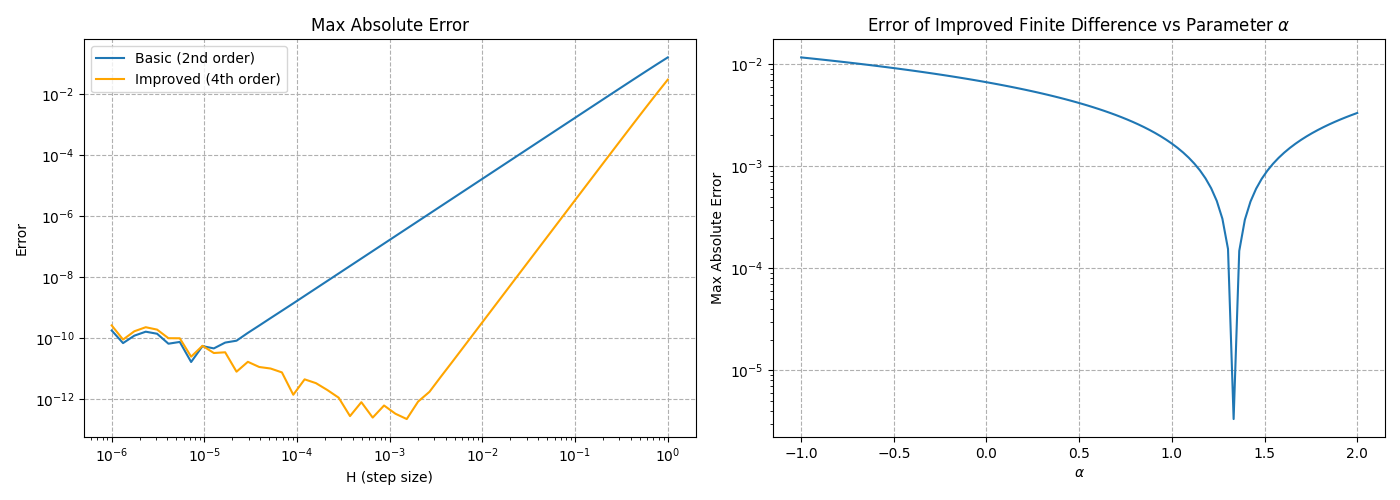
\includegraphics[scale=0.43]{img/finite-diff/finite-difference.png}
    \caption{Left pane: Approximation error for second-order and fourth-order schemes.
        For small values of $H$, round-off errors dominate.
        Right pane: Approximation error vs. $\alpha$ in the improved finite difference scheme ($H = 0.1$).
        Note that the scheme is fourth-order accurate only for $\alpha = 4/3$ (cusp in the graph).}
    \label{fig:finite-diff-accuracy}
\end{figure}

We can alternatively define the finite difference operators in terms of the delta function to get rid of the dependence on the differenced function. (Technically, the resulting quantities are functions rather than operators.)
Consider for example the two-point finite difference in \autoref{eq:two-point-central-diff}.
The definition can be generalized beyond mesh points by letting
\begin{equation*}
    D_j(\phi)(\mathbf{x}) = -\frac{\phi(\mathbf{x} + H \mathbf{e}_j)-\phi (\mathbf{x} - H \mathbf{e}_j)}{2H} = -\int \left[ \frac{\delta(\mathbf{x} + H\mathbf{e}_j - \mathbf{x}') - \delta(\mathbf{x} - H\mathbf{e}_j - \mathbf{x}')}{2H} \right]\phi(\mathbf{x}')d\mathbf{x}',
\end{equation*}
where $\mathbf{e}_j$ is the $j$-th standard basis vector.
This motivates us to define
\begin{equation}\label{eq:two-point-central-diff}
    D_j(\mathbf{x}) = \frac{\delta(\mathbf{x} + H\mathbf{e}_j - \mathbf{x}') - \delta(\mathbf{x} - H\mathbf{e}_j - \mathbf{x}')}{2H}
\end{equation}
and
\begin{equation}\label{eq:four-point-central-diff}
    D_j(\mathbf{x}) = \frac{\delta(\mathbf{x} + H\mathbf{e}_j - \mathbf{x}') - \delta(\mathbf{x} - H\mathbf{e}_j - \mathbf{x}')}{2H} + (1-\alpha)\frac{\delta(\mathbf{x} + 2H\mathbf{e}_j - \mathbf{x}') - \delta(\mathbf{x} - 2H\mathbf{e}_j - \mathbf{x}')}{4H}
\end{equation}
as the two-point as four-point finite difference operators respectively.

If $\phi$ denotes the gravitational potential, then the field $\mathbf{g}$ is approximated at mesh point $\mathbf{x}_\mathbf{p}$ as
\begin{equation*}
    \mathbf{g}(\mathbf{x}_\mathbf{p}) = -\mathbf{D}(\phi)(\mathbf{x}_\mathbf{p}).
\end{equation*}

\subsection{Interpolation}
The value of the field strength $\mathbf{g}(\mathbf{x})$ at the position particle's position $\mathbf{x}$ is calculated by interpolating the values of $\mathbf{g}$ from the neighboring mesh-points.
Formally,
\begin{equation*}
    \mathbf{g}(\mathbf{x}) = \sum_\mathbf{p} W(\mathbf{x} - \mathbf{x}_\mathbf{p}) \mathbf{g}(\mathbf{x}_\mathbf{p}).
\end{equation*}
In practice, there is no need to sum over all mesh points.
Instead, we use an algorithm analogous to \autoref{alg:density-assignment} to only include the cells with non-zero contribution to the sum.
The method is illustrated in \autoref{alg:interpolation}.
\begin{algorithm}
    \caption{Field strength interpolation}\label{alg:interpolation}
    \begin{algorithmic}[1]
        \ForAll {particle $i$}
        \ForAll {cell $\mathbf{q}$ in $\mathcal{C}_S(\mathbf{x}_i)$}
        \State $\mathbf{g}(\mathbf{x}_i) \gets \sum_\mathbf{q} W(\mathbf{x}_i - \mathbf{x}_\mathbf{q}) \mathbf{g}(\mathbf{x}_\mathbf{q})$
        \EndFor
        \EndFor
    \end{algorithmic}
\end{algorithm}
It is important to note that in order to retain correct physical behavior, the interpolation and mass assignment schemes must use the same shape to represent the particles.
The procedure in \autoref{alg:interpolation} is trivially parallelized by converting the sequential loop into a parallel one.

The procedures of density assignment and interpolation presented in \autoref{alg:density-assignment} and \autoref{alg:interpolation} are high level description.
More concrete formulations suitable for direct use in an implementation are given in \cite{Hockney1988} and \cite{Kravtsov2002PM}.

\subsection{Code units}
Implementation of the PM (and \PThreeM{}) methods can be simplified by switching to a system of dimensionless units, often called \textit{code units}.
The natural units of time and length in a PM simulation are $H$ and $DT$, respectively.
Hence, length in a PM code is conveniently expressed in terms of multiples of $H$, and similarly time intervals are given as a multiple of $DT$, i.e. the conversion relations are
\begin{equation*}
    x' = \frac{x}{H} \quad \text{and} \quad t' = \frac{t}{DT}.
\end{equation*}
From there, it follows that
\begin{equation*}
    v' = \frac{DT}{H}v \quad \text{and} \quad a' = \frac{DT^2}{H}a.
\end{equation*}
The expected relation $\mathbf{g}' = -\nabla' \phi'$ leads to the definition $\phi' = (DT^2 / H^2)\phi$.
By stipulating that we have $\nabla'^2\phi = \rho'$, we get $\rho' = DT^2 \cdot 4\pi G\rho$, $m' = (DT^2\cdot 4\pi G / H^3) m$, and $G' = 1/(4\pi)$.

\subsection{Properties of the calculated field}
The accuracy of a simulation using a PM code depends on a variety of factors.
The user can decide to use any combination of the following elements that parameterize the program:
\begin{itemize}
    \item mass assignment and interpolation scheme: NGP, CIC, TSC, or possibly any other scheme from the infinite hierarchy described in \autoref{subsec:mass-assignment};
    \item convolution with the Green's function derived from the discretized Laplacian (\autoref{eq:dft-transformed-phi}) or the ``poor man's solver'' (\autoref{eq:poor-mans-poisson-solver});
    \item gradient approximation: two-point or four-point finite difference;
    \item grid resolution: number of meshpoints in each dimension.
\end{itemize}
In this subsection we analyze these choices have in from two different angles.
We first focus on the properties of the field produced by a single source which gives insight into the behavior of the simulation on the basis of pair-wise interparticle interaction.
Then, we analyze the global error in force calculation by comparing the PM-calculated forces acting on all particles in a typical simulation with forces produced by the PP method.

\subsubsection{Local picture}
The field produced by the PM method is neither homogenous nor isotropic.
Anisotropy can be observed by measuring the field generated by a particle in two different directions.
In \autoref{fig:pm-field-properties}, the field strength calculated using the PM method (with the Green's function derived from discrete Laplacian) due to a single source at $x = H$ is shown in two variants: when measured along the $x$-axis (blue line) and the $x=y$ line (orange line).
The difference between these two graphs illustrates anisotropy of the calculated field.
The figure also shows the field strength measured along the $x$-axis when the source was shifted by $H/2$ in the $-x$ direction (green line).
Its deviation from the case when the source was placed at $x=H$ (the blue graph) exemplifies inhomogeneity of the field computed using the PM method.
\begin{figure}[htp]
    \centering
    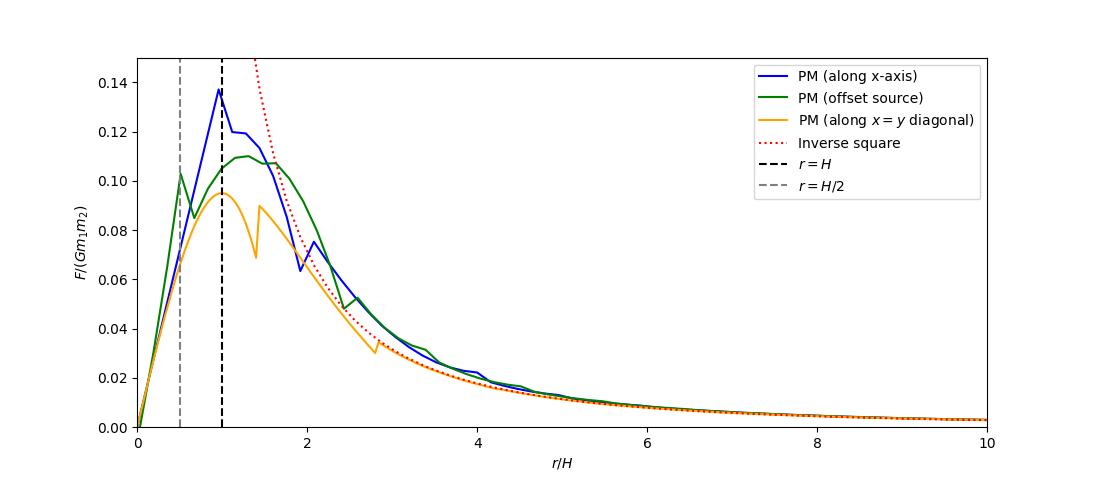
\includegraphics[scale=0.55]{img/pm/pm-field-combined.png}
    \caption{Anisotropy and inhomogeneity of the field as calculated by the PM method (TSC assignment, second order finite difference).}
    \label{fig:pm-field-properties}
\end{figure}
As expected, the PM-calculated approximation gets better with increasing distance from the source;
the inverse-square law is reproduced accurately for $r \gtrsim 4H$.

The single-source case analysis can be extended by considering the effect of choice of finite difference and mass assignment schemes on the relative error between the actual and approximated field strength.
\autoref{fig:pm-combined} shows a comparison of (a) the relative error as a function of distance from the source for PM with second-order and fourth-order finite differences, and (b) the field strength computed using different mass assignment schemes discussed in \autoref{subsec:mass-assignment}.
\begin{figure}[htp]
    \centering
    \begin{subfigure}[t]{0.48\textwidth}
        \centering
        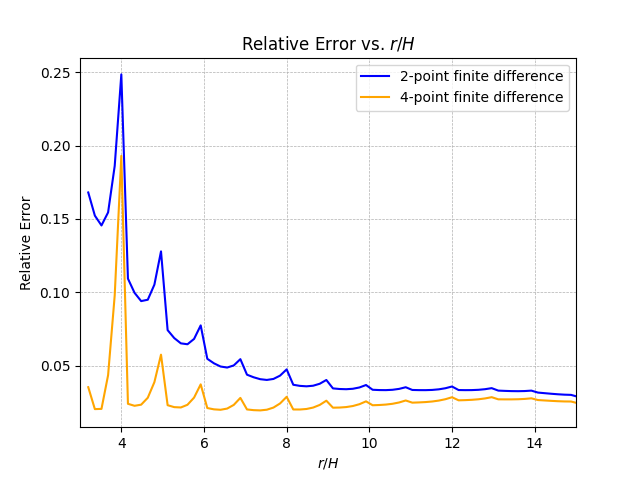
\includegraphics[width=\linewidth]{img/pm/pm-finite-diff-err.png}
        \caption{Relative error of field strength approximation in different PM variants.}
        \label{fig:pm-finite-diff-err}
    \end{subfigure}
    \hfill
    \begin{subfigure}[t]{0.48\textwidth}
        \centering
        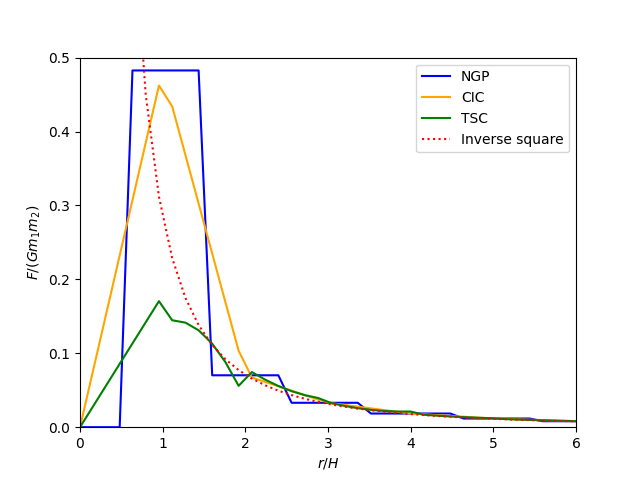
\includegraphics[width=\linewidth]{img/pm/pm-mass-assignment.png}
        \caption{Field strength calculated with the PM method using different assignment schemes.}
        \label{fig:pm-mass-assignment-field-strength}
    \end{subfigure}
    \caption{Comparison of PM method performance. (a) Relative error due to finite difference accuracy. (b) Effect of mass assignment schemes on computed field strength (4-point finite difference).}
    \label{fig:pm-combined}
\end{figure}
The conclusion that can be drawn from \autoref{fig:pm-combined} is that, as expected, the TSC mass assignment scheme and the four-point finite difference yield best results.

The field produced by the PM method using the ``poor man's'' potential solver is similar to the variant employing the discretized Laplacian Green's function described above.
\begin{figure}[htp]
    \centering
    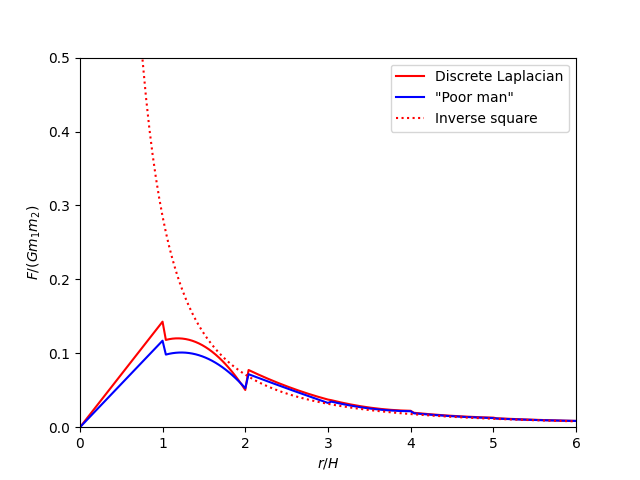
\includegraphics[scale=0.55]{img/poor-man-vs-laplacian.png}
    \caption{Field obtained potential calculated by the ``Poor man's Poisson solver'' vs. when using \autoref{eq:dft-transformed-phi}.}
    \label{fig:pm-poor-man-vs-laplacian}
\end{figure}

\subsubsection{Global picture}\label{subsubsec:pm-global-picture}
To calculate the global approximation error of a PM simulation, we calculated the average of relative differences over all particles ($N=10{,}000$ in this case) between the forces produced by the PM method and the exact result obtained using the PP method.
More precisely, we the error was defined as
\begin{equation}\label{eq:force-avg-relative-err}
    \frac{1}{N}\sum_{i} \frac{|\mathbf{F}_i^\text{approx.} - \mathbf{F}_i^\text{PP}|}{|\mathbf{F}_i^\text{PP}|}.
\end{equation}
The result, for different grid resolutions, is shown in \autoref{fig:pm-global-err-lap} ( $30 \leq N_g \leq 70$).
For the purposes of this test, the particle positions were generated according to the uniformly decreasing density disk model.
\begin{figure}[htp]
    \centering
    \begin{subfigure}[t]{0.48\textwidth}
        \centering
        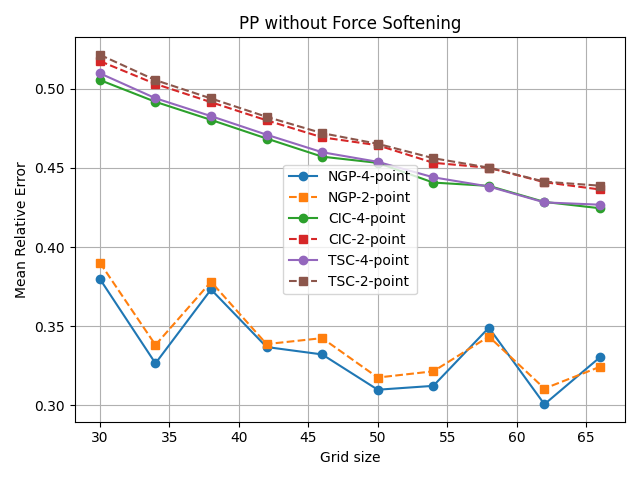
\includegraphics[width=\linewidth]{img/pm-global-err.png}
        \caption{PP calculation without force softening.}
        \label{fig:pm-global-err-lap-no-soft}
    \end{subfigure}
    \hfill
    \begin{subfigure}[t]{0.48\textwidth}
        \centering
        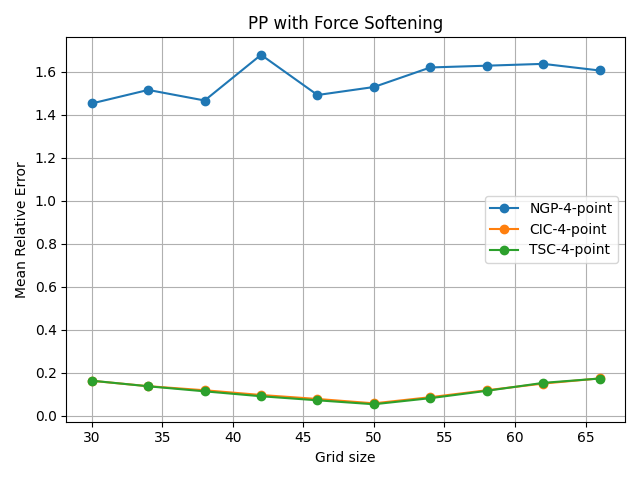
\includegraphics[width=\linewidth]{img/pm-global-err-soft.png}
        \caption{PP calculation with force softening.}
        \label{fig:pm-global-err-lap-soft}
    \end{subfigure}
    \caption{Average force approximation error in the PM method (discrete Laplacian solver).}
    \label{fig:pm-global-err-lap}
\end{figure}
As can be seen in \autoref{fig:pm-global-err-lap-no-soft}, for each of the assignment schemes, the error is minimized for the four-point difference, as expected.
A more surprising result is that the errors are seemingly greatest for the TSC assignment scheme.
This is easily explained by considering the graphs in \autoref{fig:pm-mass-assignment-field-strength}.
As can be seen there, the TSC assignment scheme gives raise to a force which accurately reproduces the inverse-square law force but at the same time it severely underestimates the force close to the source.
This behavior is expected since it stems from the mass of any individual particle being spread between multiple cells.
The CIC and NGP schemes on the other hand, do not reproduce the actual force with the same level of accuracy but the underestimation close the source is not as severe as in the case of the TSC scheme.
In some applications, for instance in the context of a galaxy simulation, this is a favorable feature of the TSC scheme.
The number of stars in a galaxy can be in the order of a trillion \cite{young2006andromeda}, whereas the number of particles in our tests is in the order of tens of thousands, giving an average of around $10^{12} / 10^{4} = 10^8$ of stars per particle.
As can be seen, it would be a serious mistake to model the force due to a single particle by the force due to a dimensionless point mass.
In such a case it is a standard practice to use a softened gravitational force instead of the one given in \autoref{eq:law-of-uni-grav} \cite{10.1046/j.1365-8711.2000.03316.x}.
By using the TSC scheme, force softening is automatically included in the calculation.
It can be argued that obtaining the smoothness properties enjoyed by the higher-order assignment schemes should be treated as tangential to softening the force.
It is for this reason, that Hockeney and Eastwood introduce the notion of \textit{force sharpening} as an additional step in the PM method in \cite{Hockney1988}.
In this modified version of the PM method, the Poisson equation takes the form
\begin{equation*}
    \nabla^2 \phi_p = \rho_p^*,
\end{equation*}
where $\rho^*_p$ is obtained from the density $\rho_p$ by solving the following system
\begin{equation*}
    1+\frac{\rho^*_{p+1} - 2\rho^*_p + \rho^*_{p-1}}{8}
    = \rho_p,
\end{equation*}
where $p$ indexes the mesh points.
In this work we do not investigate this matter further nor do we implement this modification in our program.

Now we return to the test whose results are presented in \autoref{fig:pm-global-err-lap}.
In the light of the above discussion, it is more reasonable to compare the quality of the results of the PM method with a \textit{softened gravitational force} defined in \cite{Zhang_2019} as
\begin{equation}\label{eq:softened-force}
    \mathbf{F}^\textrm{soft}_{ij} = -G\frac{m_i m_j}{(r_{ij}^2 + \epsilon^2)^{3/2}}\mathbf{r}_{ij}.
\end{equation}
The relative difference between the softened-forces and the PM-calculated ones is shown in \autoref{fig:pm-global-err-lap-soft}.
The \textit{softening length} in the PP method was set at $\epsilon = H$ in each run of the test, so that it roughly matches the softening ``induced'' by the PM method (cf. \autoref{fig:pm-mass-assignment-field-strength}).

\subsection{Implementation}
\subsubsection{CPU variant}
The most computationally involved step of the PM method is the happens in the potential solver.
As explained in \autoref{subsec:solving-the-field-equation}, in our implementation we solve the Poisson equation for the potential using the convolution method.
This involves taking the DFT of the grid-defined density and later the inverse DFT of the product of transformed Green's function and the transformed density.
Since the number of grid points in a typical grid can be of the order of a million, choosing the right implementation of the FFT is of paramount importance.
We tried incorporating a handful of popular C++ FFT libraries into the program and out of those considered, FFTW (\url{https://www.fftw.org/}) and kissfft (\url{https://github.com/mborgerding/kissfft}) provided best performance.
The running times for FFT and inverse FFT stages of the algorithm using each of the libraries are shown in \autoref{fig:cic-shape}.
\begin{figure}[htp]
    \centering
    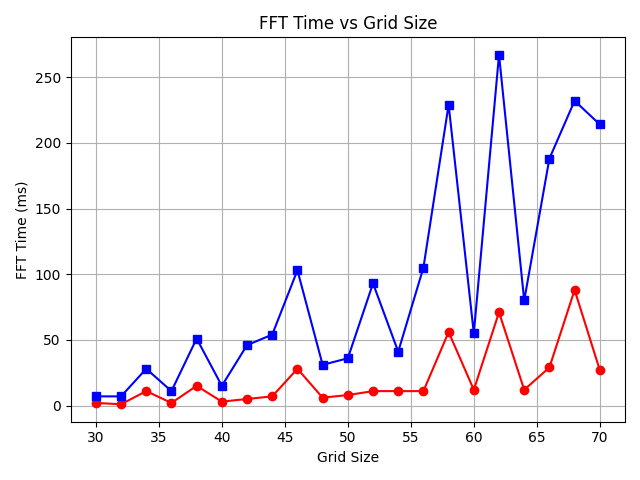
\includegraphics[scale=0.5]{img/fft_time.png}
    \caption{Time needed to perform the DFT and inverse DFT using kissft and FFTW libraries.
        The total grid size in the test was $(2N_g)\times (2N_g) \times N_g$, where $N_g$ is labeled as ``Grid Size'' on the horizontal axis in the graph.}
    \label{fig:fft-time}
\end{figure}
As we can see, FFTW considerably outperformed kissfft, with the former achieving an average five-fold speedup over the latter.
Interestingly, most spikes in the running time, taking place for certain grid sizes

As noted in \autoref{subsec:mass-assignment}, parallelization of the mass assignment step which involves ``spreading'' the mass due to a particle over nearby cells, requires synchronization to avoid data races.
The above requirement can be fulfilled by using mutexes or atomic operations.
Traditionally, atomic RMW operations were supported by the C++ standard library only for the integer types, however recently C++20 introduced atomic RMW operations on floating point numbers (see \url{https://en.cppreference.com/w/cpp/atomic/atomic.html}).
We conducted a simple benchmark on Intel Core i7-9750H CPU (three threads concurrently incrementing a global variable) to compare the performance of both approaches.
The benchmark indicated that guarding the critical section with a mutex was around two times faster than using atomic operations.
However, the same test run on a system with a different processor indicated that using atomic counter offers better performance, which shows that more careful benchmarking would be needed to reach a definite conclusion.

\subsubsection{GPU variant}
As explained before, the mass assignment, field calculation at mesh points, and interpolation steps of the PM method are embarrassingly parallel.
For this reason rewriting the PM code for the GPU does not pose much difficulty.
In our implementation we used CUDA C++ language extension to implement the method on the GPU.
A thorough introduction to the arcana of programming NVIDIA GPU devices is given in \cite{nvidia2025cuda}.
In this work, we only remark on the aspects directly related to our use case.

The memory hierarchy of a GPU (also referred to as the \textit{device}) is organized into three main levels:
\begin{enumerate}
    \item global memory (accessible by all threads as well as \textit{host} (CPU); high latency),
    \item shared memory (accessible by threads in the same threadblock typically up to 48 KB; very low latency),
    \item local storage (per thread storage in the form of registers managed by the compiler).
\end{enumerate}
We recognized that one step of the PM method that could potentially benefit from transferring data to shared memory is the gradient calculation step.
For example, if the 2-point finite difference approximation to the Laplacian is used, the potential from six cells needs to be fetched from memory.
At the same time, there is an overlap between the potential data read by threads working on adjacent mesh cells.
Thus, theoretically, fetching the potential data into shared memory could have positive impact on performance.
However, our tests for the 2-point approximation, performed at early stages of the development of the program did not indicate significant improvement in the running time of the algorithm and this optimization path was not explored further.

A major performance bottleneck in the GPU implementation is transferring the data between host and device.
These data transfers are necessary if one wishes to record the state of the simulation after each timestep.
If only the final state of the simulation is of interest, then the PM method can execute entirely on the device transferring the data to the host only once after the final iteration of the simulation.
This is the scenario that we assumed for the purpose of comparing the CPU and GPU implementation.
The results of the test for different particle numbers are shown in \autoref{fig:cpu-vs-gpu-pm}.
\begin{figure}[htp]
    \centering
    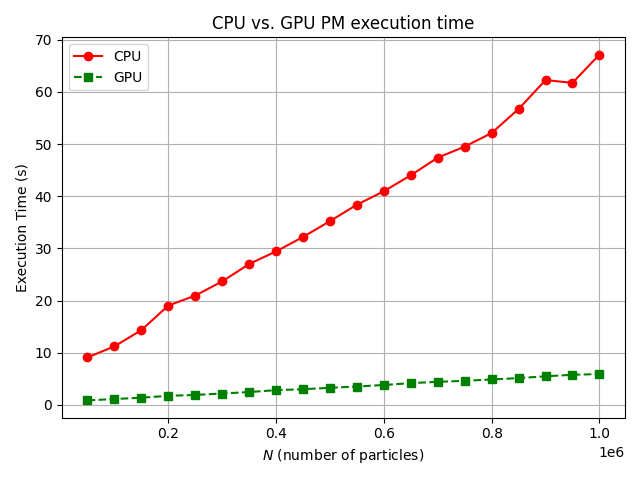
\includegraphics[scale=0.6]{img/cpu-vs-gpu.png}
    \caption{PM method: CPU and GPU implementation running time comparison.}
    \label{fig:cpu-vs-gpu-pm}
\end{figure}
In the test, the computational domain was split into $64\times 64 \times 32$ cells, and the simulation was run for 200 iterations.
Both plots in the figure exemplify linear complexity of the PM method, with the GPU implementation providing 1200\% speedup over the CPU version.